\chapter{Introduction to variable stars}

The First Nations people of Australia have lived here for over 65\,000 years and have oral traditions that highlight their understanding of variations in the brightness of stars. In particular, this knowledge encompasses the naked eye observations of the decades-long variability of three of the brightest southern stars, known in Western astronomy as Aldebaran, Betelgeuse and Antares \citep{hamacher_observations_2018}. In contrast to this, Western astronomy abode by the conclusions of Aristotle (350 BCE) that stars are static, with the exception of observations of supernovae, for almost two thousand years. 

David Fabricius' observations of the variable star Mira in 1596, later revealed to have a periodic brightness change of 332\,days, confirmed for modern astronomy that stars could indeed be variable \citep{hoffleit_history_1997}. Our understanding of stellar variability has progressed significantly in the last century; both in terms of the range of stars where we observe variability and the explanation for its existence. Henry Russell's 1918 address on variable stars stated `almost all variable stars are... giants...' with variability being a characteristic of the early life of a star \citep{payne-gaposchkin_development_1978}. These variable stars were limited to approximately 1\,700 examples divided into five classifications; novae, long-period variables (like Mira), irregular variables, Cepheids, and eclipsing stars. 

Today, the General Catalog of Variable Stars \citep{samus_general_2017} contains 117 distinct classes of variable objects, almost all belonging to the subset of variable stars and including stars of all evolutionary stages. This progress is the result of technological advances, from observations by eye to the adoption of photographic plates and finally modern Charge-Coupled Devices (CCDs), providing increased precision and accuracy in photometric measurements.

\todo{Motivation for studying variable stars}


%----------------------------------------------------------------------------------------------------------------------------------------------------------------
%----------------------------------------------------------------------------------------------------------------------------------------------------------------


\section{Classification}

The physical phenomenon producing observed variances in the photometric brightness of an object can be used to create a classification scheme for variables. \citet{eyer_variable_2008} have produced a classification tree (reproduced here as Figure \ref{fig:variability_tree}) based on four levels of differentiation: (1) intrinsic or extrinsic variability, (2) the type of object that is variable, (3) the physical phenomenon causing the variability, and (4) the grouping of similar variable objects.

\begin{figure}[htbp]
    \centering
    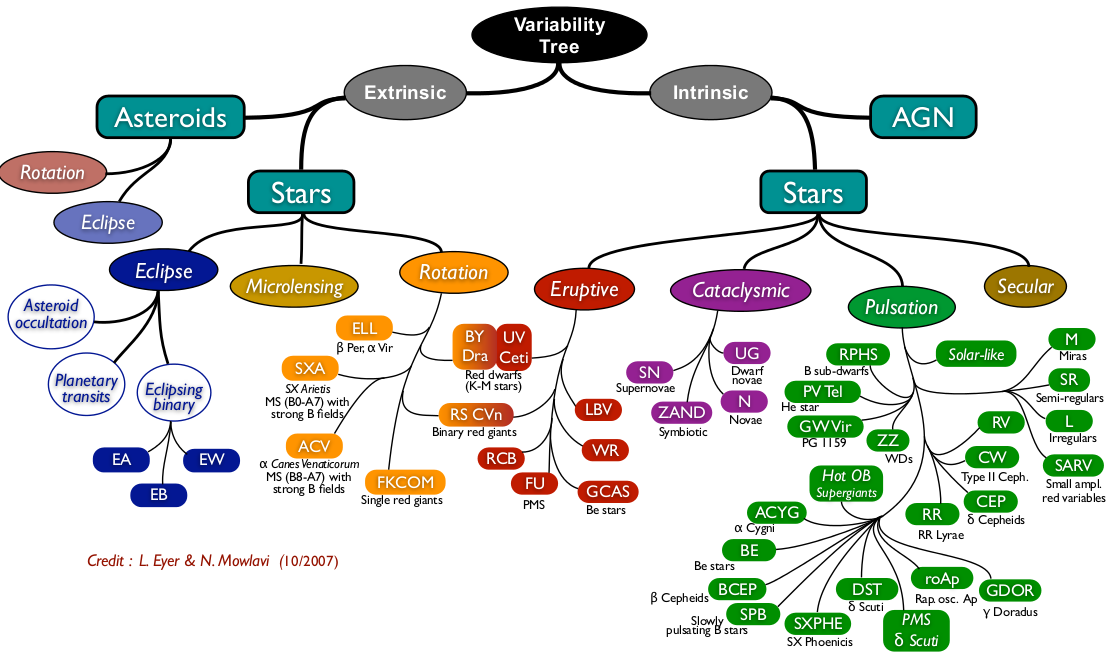
\includegraphics[height=0.78\linewidth,angle=-90]{Chapter1/variable_EyerMowlavi08.png}
    \caption[Variability classification tree]{Reproduction of \citet{eyer_variable_2008} classification tree of different variability types. Variable stars are the focus of this thesis so other variable objects at the second division level will not be discussed.}
    \label{fig:variability_tree}
\end{figure}

At the first division, intrinsic variables refer to stars where the variability is due to a physical process occurring withing the star itself. Extrinsic variability refers to cases where the geometry of the observations results in variability. This thesis is only concerned with variable stars and other variable object types will not be discussed, so the second division is not considered here. 

The third differentiation is based on the specific physical phenomenon at the object that causes the variability. The largest intrinsic category is stellar pulsations with almost all stars now known to exhibit this form of variability. Stellar rotation showing different regions of the surface, and eclipsed stars make up the most common examples of extrinsic variability. At the lowest level the different variable classifications are clustered together based on similar variability characteristics.

The classes are not all distinct at the lowest level, with some continuous transitions as the star passes from one evolutionary stage to another. To further complicate this process, variable stars may show signatures of more than one of these sources. (e.g. An eclipsing binary with a rotating red giant companion and a transiting exoplanet could show signatures belonging to four of these categories.) 

Detecting stellar variability at the lowest levels relies on accurate, and precise photometric measurements with continuous observations over long time periods.
There have been many missions and surveys over the past two decades dedicated to obtaining multi-epoch photometry including both ground-based missions (e.g. \textsc{Macho}, \textsc{Ogle} (I, II, and III), LSST, PanSTARRS, SONG, and HAT) and space-based telescopes (e.g. \Kepler, \Gaia, MOST, and \textsc{CoRoT}).

%Discussion & CRITIQUE of diagram. Bias etc
This figure was produced primarily for the classification of variables found in the \Gaia~mission and so is biased towards the broader classification of variable objects. Solar-like oscillators are combined into a single object classification in this schema, yet they account for a large proportion of the pulsating stellar variable population and are diverse in nature. This classification further separates stellar objects at different evolutionary stages into completely separate classifications. For example, evolved red giant stars showing Mira-like pulsations show no common branches with the solar-like oscillators they evolved from.

The introduction of photometric space-based telescopes to study solar-like stars (e.g MOST) and to search for exoplanets around them (e.g \Kepler, \textsc{CoRoT}, and TESS) have provided high precision photometry with the quality and quantity of data necessary to detect these oscillations unambiguously \citep{stello_detection_2010}. This data has revolutionised the study of stellar variability since the publication of the variability classification scheme above (e.g \citet{chaplin_asteroseismic_2010}  and \citet{basu_determination_2010}). 
\todo{CHECK THESE REFERENCES!!}



Importance of variable stars
    - Pulsating stars
        - Interior of stars (asteroseismology)
    - Eclipsing binaries
        - Masses of stars
    - Transits
        - Exoplanet hunting
    - Rotation
        - Splitting of modes
        - Spots
        - Magnetic field investigations

\subsection{Pulsating stars}

Pulsating variable stars are particularly important in expanding our understanding of stellar processes, interiors, and evolution. These stars are intrinsic variables; physical changes within the star are responsible for their variability. 

Different types of pulsating stars
Processes and Mechanisms - kappa, stochastic, convective blocking, tidal excitation
HR Diagram defined, show different variables and how they correspond to different regions.
Importance of variable stars
How we measure pulsations - asteroseimology.

Eddington - How can we see inside stars.
Asteroseismology. As such intrinsically variable stars are interesting
Almost all stars are intrinsically variable we have found as the detection limit is lowered.


% Pulsating variable stars are intrinsic variables as their variation in brightness is due to a physical change within the star. In the case of pulsating variables this is due to the periodic expansion and contraction of the surface layers of the stars. This means the star actually increases and decreases in size periodically. The different types of pulsating variable are distinguished by their periods of pulsation and the shapes of their light curves. These in turn are a function of the mass and evolutionary stage of a given star.

% The study of pulsating variables is of great importance to astronomers. Analysis of light curves provides vital information about the interior processes in stars. Perhaps their most valuable property of many types of pulsating variables is a direct relationship between the period of pulsation and their luminosity. This in turn allows us to determine the distance to such stars and is discussed in more detail on the next page.

% As with non-pulsating variables, there are several types of pulsating stars and some of the key types are described briefly below.


% We observe pulsational variability in stars of all types.  exhibit pulsational variations, driven by one of two oscillation mechanisms. % There are two main processes which excite stellar oscillations, the heat-engine mechanism
% (Eddington, 1926), and stochastic excitation (e.g. Unno, 1964). The heat-engine mecha-
% nism was first proposed by Eddington who considered pulsating stars as thermodynamic
% heat engines where radial oscillations result from sound waves resonating in the stellar
% interior. In this mechanism, a shell of stellar mass loses its support against the gravita-
% tional field of the star and collapses towards the centre of the star. This collapse results
% in the compression of the shell s mass which in turn restricts the radiation transfer from
% the stellar core and increases the shell s temperature. This temperature increase causes a
% respective increase in the pressure acting on the shell, forcing it to expand. As it expands,
% 1the radiation pressure decreases and the shell cools down forcing the shell to collapse once
% more.

% driving these  The Hertzsprung-Russel (HR) Diagram 

% HR Diagram is a tool that can be used to show the pulsating stars.

% Murphy Thesis
% The A stars exhibit a range of pulsation phenomena. This is where many of the
% classical pulsators—those driven by the ‘heat-engine’ mechanism—are found. Under
% this mechanism, first proposed by Eddington (1917), a layer heats up on compression,
% increasing the region’s opacity and driving radius expansion. The expanded region
% later cools, causing an opacity drop and re-compression. The dependence on opacity
% has lead to the mechanism being known as the opacity-, or simply κ-mechanism.
% The RR Lyrae variables, rapidly oscillating Ap (roAp) stars and δ Scuti stars are all
% examples of A stars driven by the κ-mechanism. Classical Cepheid variables are also
% driven by the κ-mechanism, but at later spectral types. The γ Doradus variables make
% up a large number of variables at early-F spectral types, but are driven by a convective-
% flux modulation mechanism (Guzik et al. 2000). Some stars show pulsations driven
% by more than one mechanism and are known as hybrids (Handler 2012).

% We will refer to pulsation modes using quantum numbers: n is the overtone or
% radial order of the mode, indicating the number of radial nodes; l is the degree, indi-
% cating the number of surface nodes; and m is the azimuthal order, with |m| indicating
% the number of surface nodes that are also lines of longitude. We shall see later that
% the sign of m indicates whether the mode is prograde or retrograde, and we use the
% convention that prograde modes have negative m values and higher frequencies in the
% observer’s frame. Pressure modes (p modes) are denoted with positive values of n,
% and gravity modes (g modes) with negative values. One sometimes writes p 1 , p 2 ,...,
% to denote the n-value of the p modes. The g modes are always non-radial, that is, they
% have l ≥ 1. Spherically symmetric stars have degenerate pulsation frequencies, in
% that all modes with the same (n, l) have the same frequency, regardless of m. Rotation
% and magnetic fields can break the symmetry and lift this degeneracy, however.

% Jason Thesis
% 1.1.1 Oscillation Mechanisms
% There are two main processes which excite stellar oscillations, the heat-engine mechanism
% (Eddington, 1926), and stochastic excitation (e.g. Unno, 1964). The heat-engine mecha-
% nism was first proposed by Eddington who considered pulsating stars as thermodynamic
% heat engines where radial oscillations result from sound waves resonating in the stellar
% interior. In this mechanism, a shell of stellar mass loses its support against the gravita-
% tional field of the star and collapses towards the centre of the star. This collapse results
% in the compression of the shell s mass which in turn restricts the radiation transfer from
% the stellar core and increases the shell s temperature. This temperature increase causes a
% respective increase in the pressure acting on the shell, forcing it to expand. As it expands,
% 1the radiation pressure decreases and the shell cools down forcing the shell to collapse once
% more.
% The κ mechanism (Eddington, 1941) is a heat-engine mechanism predominantly ob-
% served in classical pulsators such as RR-Lyrae, δ-Scuti and Cepheid stars which results
% from changes in opacity within the star. Ionisation of helium and hydrogen within the
% stellar envelope, resulting from the absorption of radiation from nuclear fusion, produces
% regions of higher relative opacity than the surrounding non-ionised layers. These zones of
% higher opacity store flux from the inner layers when compressed (Zhevakin, 1958). This
% energy absorption causes the layers to expand towards their equilibrium point, resulting
% in the release of the temporarily-stored energy. The layer however continues expanding
% beyond its equilibrium position as it cools decreasing its opacity and allowing more flux
% to escape, inducing oscillations around the equilibrium (King and Cox, 1968).
% Variable stars which exhibit solar-like oscillations such as red giants, cool sub-giants
% and lower main sequence stars are characterised by stochastically excited oscillations.
% These randomly-excited oscillations evolve from turbulence within a thick, convective
% layer in the outer envelope of the star. The turbulent driving force for these oscillations
% occurs in the region of this convective layer where the time scales for the pulsations and
% convection are closely correlated (Handler, 2013). For such a convective layer to form,
% the stars must be cooler than the red edge of the classical instability strip where classical
% pulsators reside (Bedding, 2011), see Figure 1.1.
% The turbulence within these variable stars perturbs the stellar structure, forming nor-
% mal modes and thus global oscillations when they coincide with standing wave frequencies.
% Despite constant convective forcing, these modes have a finite lifetime resulting from de-
% structive interference with out-of-phase stochastic excitations. Any oscillations which do
% not correspond to normal modes decay rapidly due to internal damping and are not ob-
% served as global oscillations. Such solar-like oscillators shall be the main topic of this
% research project.
% Photometry is one analytical technique utilised for detecting and investigating stellar
% oscillations and relies upon on the detection of variations within the stellar luminosity
% measurements to detect source variability. Stellar luminosity is affected by a combination
% of both the temperature and radius of the star. The particular characteristic which
% dominates this interaction depends on the specific wavelength regime and the type of star
% being considered. For red giant stars for instance, changes in the stellar radius tend to
% dominate this relation.

% ----

\begin{figure}[htbp]
    \centering
    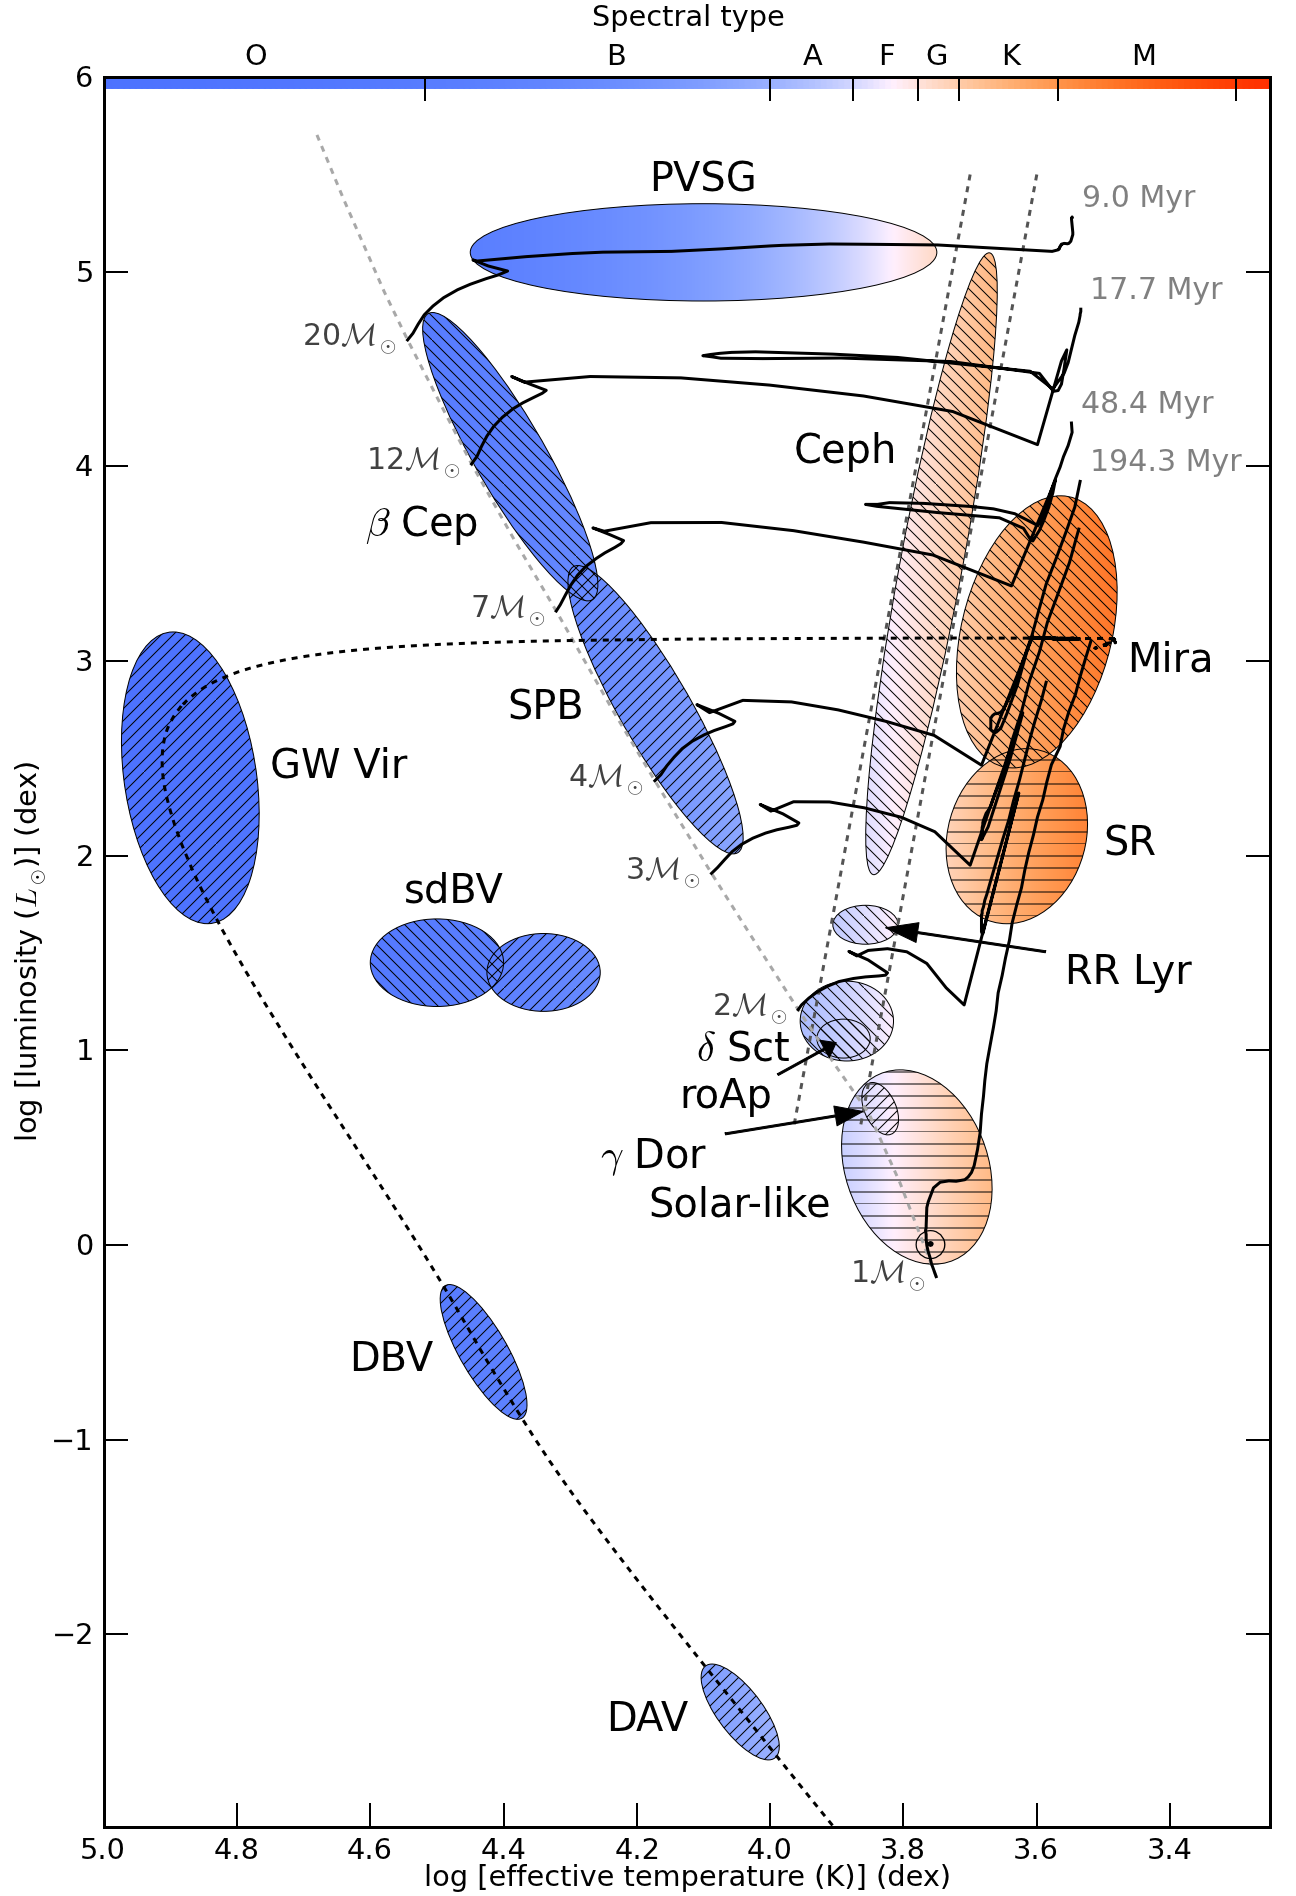
\includegraphics[height=0.5\paperheight]{Chapter1/HR_pulsational.png}
    \caption[Pulsational Hertzsprung-Russell Diagram]{}
    \label{fig:HRdiag}
\end{figure}

HR diagram showing variable star regions - P. Begroote, P. Papics

Oscillation mechanisms

% Excitation mechanisms
%\kappa -mechanism
% Main article: Kappa mechanism
% Under fairly specific conditions, some stars have regions where heat is transported by radiation and the opacity is a sharply decreasing function of temperature. This opacity bump can drive oscillations through the {\displaystyle \kappa } \kappa -mechanism (or Eddington valve). Suppose that, at the beginning of an oscillation cycle, the stellar envelope has contracted. By expanding and cooling slightly, the layer in the opacity bump becomes more opaque, absorbs more radiation, and heats up. This heating causes expansion, further cooling and the layer becomes even more opaque. This continues until the material opacity stops increasing so rapidly, at which point the radiation trapped in the layer can escape. The star contracts and the cycle prepares to commence again. In this sense, the opacity acts like a valve that traps heat in the star's envelope.

% Pulsations driven by the {\displaystyle \kappa } \kappa -mechanism are coherent and have relatively large amplitudes. It drives the pulsations in many of the longest-known variable stars, including the Cepheid and RR Lyrae variables.

% Surface convection
% In stars with surface convection zones, turbulent fluids motions near the surface simultaneously excite and damp oscillations across a broad range of frequency.[2][3] Because the modes are intrinsically stable, they have low amplitudes and are relatively short-lived. This is the driving mechanism in all solar-like oscillators.

% Convective blocking
% If the base of a surface convection zone is sharp and the convective timescales slower than the pulsation timescales, the convective flows react too slowly perturbations[clarification needed] that can build up into large, coherent pulsations. This mechanism is known as convective blocking[4] and is believed to drive pulsations in the {\displaystyle \gamma } \gamma  Doradus variables.[5]

% Tidal excitation
% Observations from the Kepler satellite revealed eccentric binary systems in which oscillations are excited during the closest approach.[6] These systems are known as heartbeat stars because of the characteristic shape of the light curves.





Variable stars in open clusters


%----------------------------------------------------------------------------------------------------------------------------------------------------------------
%----------------------------------------------------------------------------------------------------------------------------------------------------------------


\section{Open clusters}

Open clusters are typically characterised as sparse, loosely gravitationally-bound stellar populations located primarily in the galactic disk \citep{friel_old_1995}. Older open clusters tend to be more densely populated, with hundreds to thousands of members, compared to younger clusters that comprise a few tens to hundreds of members. These older open clusters also tend to be located at greater distances from the galactic disc, where the probability of collisions with large molecular clouds, that disperse cluster members among the galactic field population, are more remote \citep{}. \todo{Get reference from pad on bookshelf/in paper box?} Tidal disruption, disc and bulge shocking, and stripping from galactic field interactions are also responsible for the dissolution of stellar cluster members into the field population \citep{marchi_search_2006}. All of these processes are most prevalent in the galactic disc.\todo{Check this statement}

Stellar cluster populations form within a single nebula and consist of coeval, isometallic, cospatial and comoving members \citep{baade_resolution_1944}, with initial stellar mass being the primary parameter that differentiates members. \citet{mould_stellar_1982} showed that the metallicity and kinematics of cluster members are unchanged by stellar and galactic evolution, making cluster members ideal probes for a wide range of astrophysical investigations (e.g stellar interiors and atmospheres \citep{}, stellar evolution \citep{kalirai_jason_s._star_2010}, cosmology \citep{}, galactic evolution \citep{de_grijs_revolution_2010}, and disk and planet formation \citep{}).

In terms of stellar evolutionary studies, the fewer free parameters required for modelling cluster members allows the analysis to be conducted as a uniform ensemble, with a few exceptions resulting from rotation, magnetic field interactions and binarity \citep{carroll_introduction_2006}. Whilst globular clusters may experience multiple stellar formation epochs, this is not the case for open clusters \citep{li_stellar_2016} that are instead well-described by a single isochrone (a composite of coeval theoretical evolutionary tracks for different initial mass values) transformed to the observational CMD regime. Photometric observations of cluster members reveal outliers from these isochrones, with binarity being perhaps the most influential cause (e.g. \citet{duquennoy_multiplicity_1991} and \citet{murphy_finding_2018}), resulting in apparent magnitudes of up to 0.75\,mag brighter for unresolved binaries.

This thesis will focus on the four open clusters located in the nominal \Kepler field of view; NGC\,6791, NGC\,6819, NGC\,6811, and NGC\,6866. These clusters span a range of ages and metallicities. Table \ref{tab:cluster_properties} presents a summary of the global cluster properties.

\subsection{NGC 6791}

From Honours: 
NGC 6791 is an open cluster located in the Lyra constellation at a distance of approximately 4.1\,kpc \citep{basu_determination_2010}. It is one of the oldest, most metal-rich open clusters with an approximate age of 8 Gyrs (\citet{grundahl_2008}, \citet{king2005}, \citet{stetson_2003}) and metallicity [Fe/H] = +0.30 \citep{boesgaard_2009}. The high metallicity of this cluster is atypical, as older stellar clusters tend to have lower metallicities than younger ones, originating from the initial chemical composition of the dust cloud they form from. The population density of cluster members is also much higher than most other open clusters and combined with its metal-rich nature has led to NGC 6791 becoming one of the most studied open clusters in the galaxy. Previous studies of this cluster have reported age discrepancies/discontinuities between cluster members with the faint white dwarf members having much younger ages of approximately 4 to 6 Gyrs compared to the average of 8 Gyrs for the majority of the cluster members \citep{Bedin2008}. Theoretical investigations however revised the calculations for white dwarf age determination and demonstrated a common age of 8 Gyrs for all cluster members investigated \citep{Garciaberro2010}. 

\subsection{NGC 6819}

NGC 6819 is an open cluster located approximately 2.16 kpc away in the Cygnus constellation (Balona et al., 2013). It is a much younger open cluster than NGC 6791 with an average stellar age of approximately 2.5 Gyrs (Kalirai et al., 2001; Rosvick and Vandenberg, 1998) and solar metallicity of [Fe/H] = +0.09 (Bragaglia et al., 2001).


\subsection{NGC 6811}
\subsection{NGC 6866}

% There are four open clusters spanning a range of ages and metallicities within the
% Kepler field of view (FOV); NGC 6791, NGC 6811, NGC 6866 and NGC 6819. Several
% membership and quantitative studies have already been conducted on these clusters based
% solely on observations of stars targeted for observation and analysis by the Kepler mission
% (Basu et al., 2011). The first clear measurements of solar-like oscillations in these cluster
% stars were detected through relative flux variations and presented by Stello et al. (2010).

% NGC 6791 is an open cluster located in the Lyra constellation at a distance of approxi-
% mately 4.1 kpc (Basu et al., 2011). It is one of the oldest, most metal-rich open clusters
% with an approximate age of 8 Gyrs (Grundahl et al., 2008; King et al., 2005; Stetson et al.,
% 2003) and metallicity [Fe/H] = +0.30 (Boesgaard et al., 2009). The high metallicity of this
% cluster is atypical, as older stellar clusters tend to have lower metallicities than younger
% ones, originating from the initial chemical composition of the dust cloud they form from.
% The population density of cluster members is also much higher than most other open
% clusters and combined with its metal-rich nature has led to NGC 6791 becoming one
% of the most studied open clusters in the galaxy. Previous studies of this cluster have
% reported age discrepancies/discontinuities between cluster members with the faint white
% dwarf members having much younger ages of approximately 4 to 6 Gyrs compared to the
% average of 8 Gyrs for the majority of the cluster members.(Bedin et al., 2008) Theoretical
% investigations however revised the calculations for white dwarf age determination and
% demonstrated a common age of 8 Gyrs for all cluster members investigated.(Garcı́a-Berro
% et al., 2010)

% NGC 6819 is an open cluster located approximately 2.16 kpc away in the Cygnus constel-
% lation (Balona et al., 2013). It is a much younger open cluster than NGC 6791 with an
% average stellar age of approximately 2.5 Gyrs (Kalirai et al., 2001; Rosvick and Vanden-
% berg, 1998) and solar metallicity of [Fe/H] = +0.09 (Bragaglia et al., 2001).
\begin{table}[h]
    \setlength\tabcolsep{10pt}
    \centering
    \begin{tabular}{lcccc}
        \hline
                        & NGC 6791 & NGC 6819 & NGC 6811 & NGC 6866 \\
        \hline
        \hline
        RA                      &  &  &  & \\
        Dec                     &  &  &  & \\
        Distance                &  &  &  & \\
        Age (Gyrs)              &  &  &  & \\
        Metallicity [Fe/H]      &  &  &  & \\
        Radius                  &  &  &  & \\
         - Core                 &  &  &  & \\
         - Tidal                &  &  &  & \\
         - Limiting             &  &  &  & \\
         Population             &  &  &  & \\
        \hline
        
    \end{tabular}
    \caption{A summary of the global properties of the four open clusters in the nominal \Kepler field of view; NGC\,6791, NGC\,6819, NGC\,6811, and NGC\,6866.}
    \label{tab:cluster_properties}
\end{table}


%----------------------------------------------------------------------------------------------------------------------------------------------------------------
%----------------------------------------------------------------------------------------------------------------------------------------------------------------

\section{Kepler}
NASA's \Kepler~space telescope was a 1.4m modified Schmidt design that completed its nominal mission between May 2009 and May 2013. It was designed primarily to detect transiting exoplanets by obtaining micro-magnitude precision photometry of approximately 150\,000 stars within its field of view. The ultimate goal was the detection of Earth-sized exoplanets in the habitable zone of solar-like stars, and the determination of the populations of such planets in the Milky Way \citep{koch_kepler_2010}.

Figure \ref{fig:KepSchema} shows a schematic diagram of the \Kepler~space telescope components; the photometer, made up of the telescope and detector, and the spacecraft itself.  The telescope included a 1.4\,m primary mirror and a 0.95\,m aperture Schmidt corrector plate focusing light onto a 95 megapixel detector at the focal plane. The spacecraft included a solar array, thermal radiator, a high-gain (Ka-band) antenna for data transmission, four reactor wheels, and thruster modules.

\begin{figure}[htbp]
    \centering
    \vspace{0.5em}
    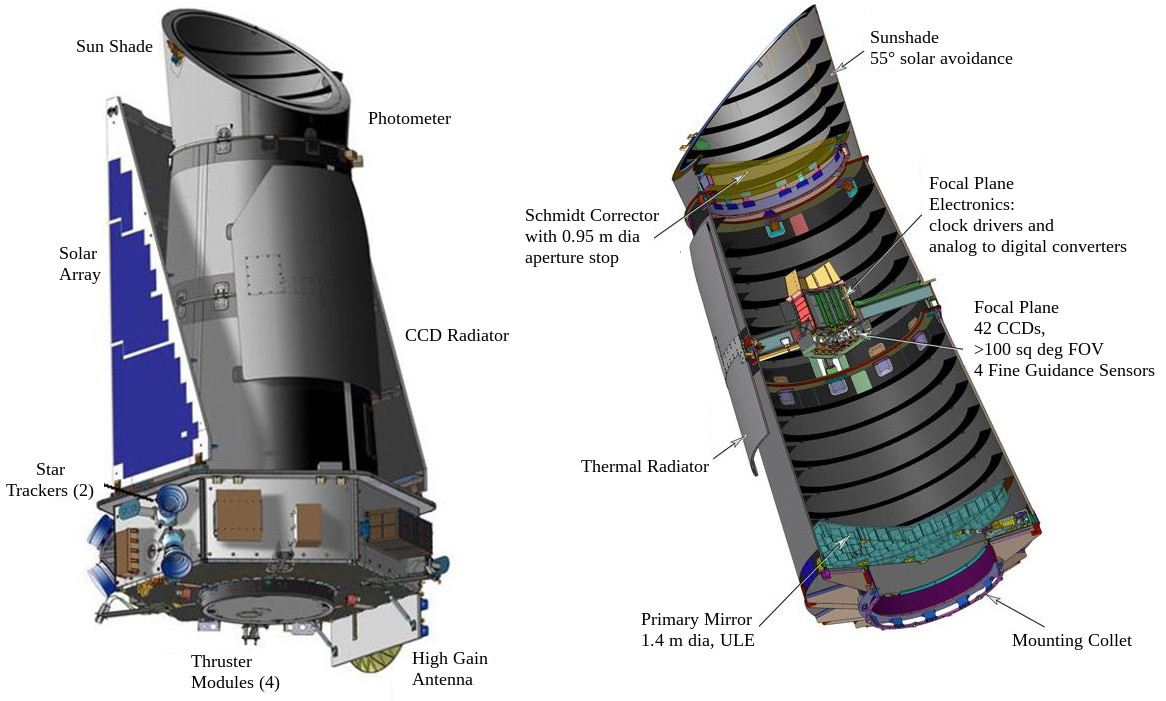
\includegraphics[width=0.9\linewidth]{Chapter1/Kepler_schema_both.jpg}
    \vspace{0.5em}
    \caption[Schema of the \Kepler~spacecraft]{Schema of the \Kepler~space telescope showing (a) The main components of the spacecraft and (b) A cutout of the photometer highlighting the internal structure including the focal plane, 1.4\,m primary, 0.95\,m schmidt corrector plate, and the positioning of the CCD detector.}
    \label{fig:KepSchema}
\end{figure}

The detector (Figure \ref{fig:Kep_detect}) was composed of 42 thinned, back-illuminated CCDs of dimensions 50\,mm $\times$ 25\,mm, arranged into 21 square modules. Each CCD had a resolution of 2200 $\times$ 1024 pixels (px) with a physical pixel size of 27 $\mu m^2$. This detector was maintained at -85\,$\degree$C via the thermal radiator to ensure near constant efficiency of the CCDs.

\begin{figure}[htbp]
    \centering
    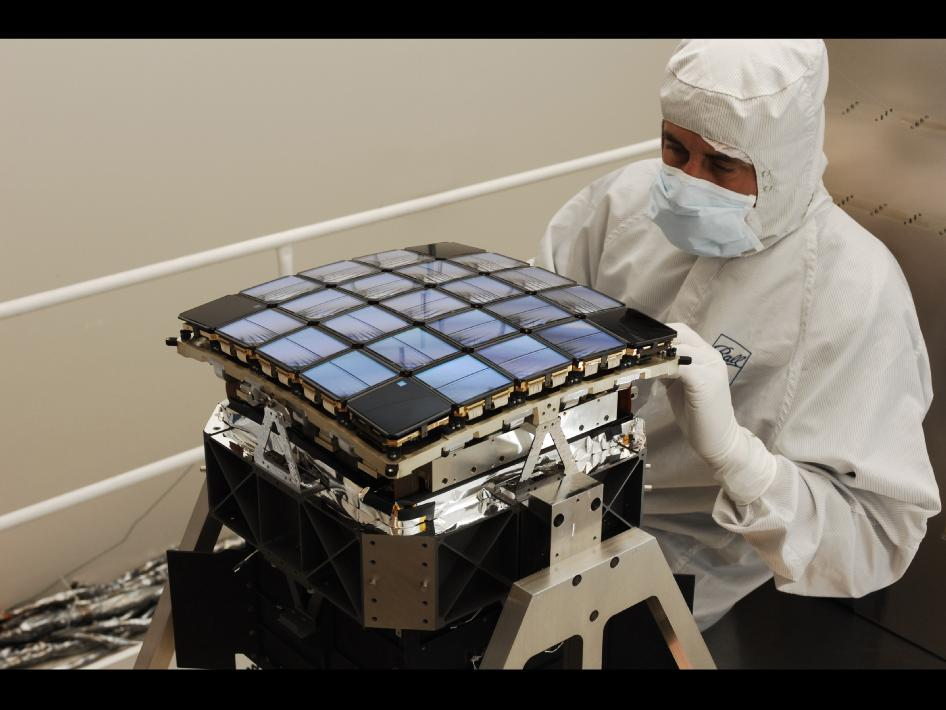
\includegraphics[width=0.45\linewidth]{Chapter1/Kepler_detector.jpg}
    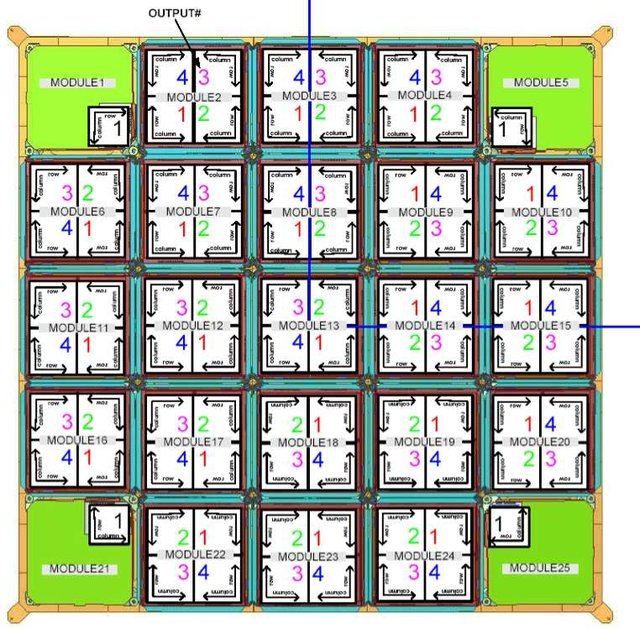
\includegraphics[width=0.45\linewidth]{Chapter1/kepCCD.jpg}
    \caption[Kepler CCD detector array prior to installation]{Left: The focal plane array assembly showing the 42 CCDs that comprised the detector at Bell Labs prior to launch. Right: A schematic of the detector module placements and identification of each module and output. Module positions 1, 5, 21, and 25 are occupied with fine guidance sensor chips.}
    \label{fig:Kep_detect}
\end{figure}

\subsection{Mission}
For the nominal mission \Kepler~maintained a 105 square degree field of view (FoV) centred between the constellations of Cygnus and Lyra, and located 13.5 degrees above the galactic plane. Figure \ref{fig:kepFoV} presents a stylised representation of the telescope's nominal FoV with stellar magnitudes represented by the size of the filled circles. The four open clusters that are present are marked by dashed lines. Note that the detector is positioned to ensure the brightest stars are focussed between the modules to minimise blooming (overexposure and charge-bleeding along CCD rows). This FoV produces a pixel scale of 3.98\,"/px. The telescope was intentionally defocussed to diffuse the light of a stellar target to 10\," to ensure the best possible photometric stability.

\begin{figure}[htbp]
    \centering
    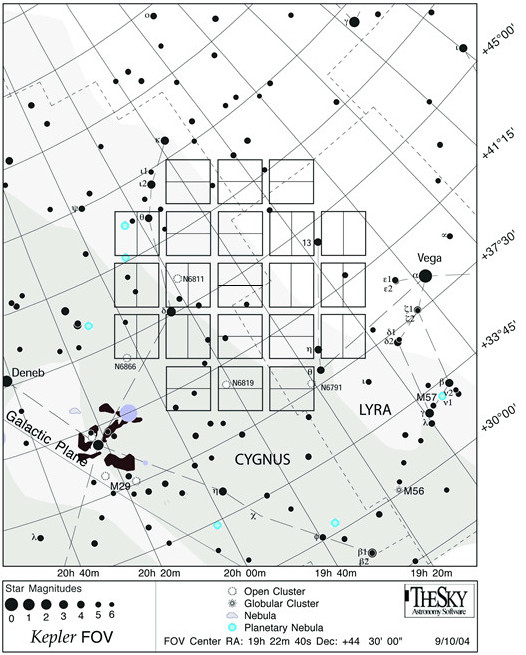
\includegraphics[height=0.32\paperheight]{Chapter1/kepFoV.jpg}
    \vspace{0.5em}
    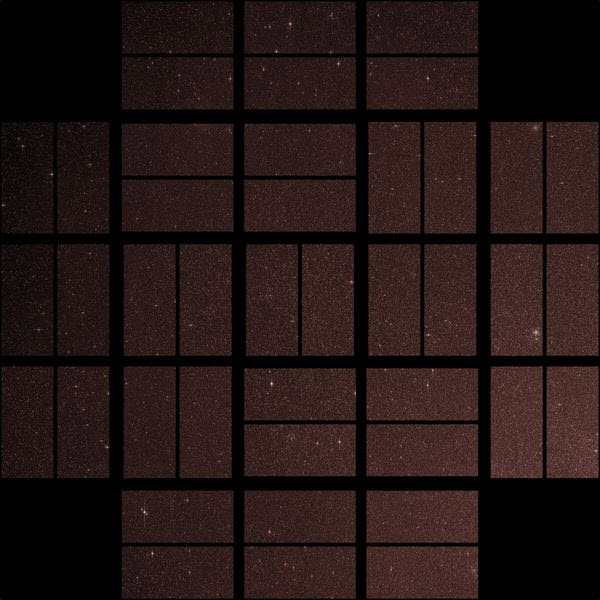
\includegraphics[width=0.45\linewidth]{Chapter1/kepFFI.jpg}
    \caption[\Kepler field of view; stylised, and full-frame image]{Left: Stylised representation of the \Kepler\, field of view between the constellations of Cygnus and Lyra. Larger filled circles represent stars of brighter magnitude. The four open clusters in the FoV are designated by dashed circles. Right: An example of the full-frame images (FFIs) of \Keplers~FoV.}
    \label{fig:kepFoV}
\end{figure}

\Kepler~occupied an Earth-trailing heliocentric orbit (ETHO) with the field of view selected to avoid Earth-shine, Moon-shine, and sunlight from entering the photometer. One of the characteristics of an ETHO are lower torques acting on the spacecraft, enabling more efficient fine-pointing control. This control is achieved through the four reactor wheels that spin up to store the angular momentum from the acting torques before being dumped through thruster burns. The orbit also required the spacecraft to rotate every 90\,days to maintain sunlight on the solar array and exposure of the thermal radiator to deep space, placing stars on different CCDs. This rotation resulted in data being divided into "quarters" at each rotation. The initial 30\,d observing run following the 10\,d engineering test but prior to the first rotation is termed quarter 1 (Q1), with the nominal mission terminating after Q17 due to the failure of a second reaction wheel. These observations provide baseline photometry for most target stars of approximately 1\,460\,days.

\subsection{Data Products}

Whilst the ETH orbit is much more fuel efficient than an Earth-centric one, the constantly increasing distance between the spacecraft and Earth limits the bandwidth available for data down-link through NASA's Deep Space Network. Full-frame images (FFIs) of \Keplers~FoV were too large to be downloaded at the cadence required for the mission's science goals, so subsets of these images were selected for down-link, with a single FFI (Figure \ref{fig:kepFoV}) downloaded every 30\,d \citep{thompson_kepler_2016}. All data products from the mission preserved pixel-level data, so subsets could be queried per pixel. Module 3 of the CCD detector failed in January 2010, so all stars that fell on this module have data gaps every four quarters that correspond to the spacecraft's rotation.

\subsubsection{Target Pixel Files}
The primary data products consisted of subsets or `postage stamps' of the CCD array output around target stars called target pixel files (TPFs) and were produced for around 150\,000 targeted stars per quarter. There were two observational cadences for the TPFs; long cadence (LC) observations with a total exposure time of 29.43\,m, and a smaller subset of approximately 500 short cadence (SC) observations with an exposure time of 58.86\,s. The LC exposures consisted of 270 CCD readout cycles (6.02\,s exposure followed by 0.52\,s readout per cycle) co-added on board the spacecraft while the SC TPFs consisted of 9 co-added cycles. These were stored in on-board memory until down-link, every 30\,days.

\subsubsection{Superstamp Images}
In addition to the primary data products, large 200 $\times$ 200\,px `superstamps', centred on the open clusters of NGC\,6791 and NGC\,6819, were downloaded at LC exposure intervals for quarters 1 to 17. Figure \ref{fig:SS} shows a typical exposure of these superstamp images for each cluster. NGC\,6819 fell on module 3 of the detector from Q2, so no superstamps are available for this cluster for Q6, Q10 or Q14.

\begin{figure}[htbp]
    \centering
    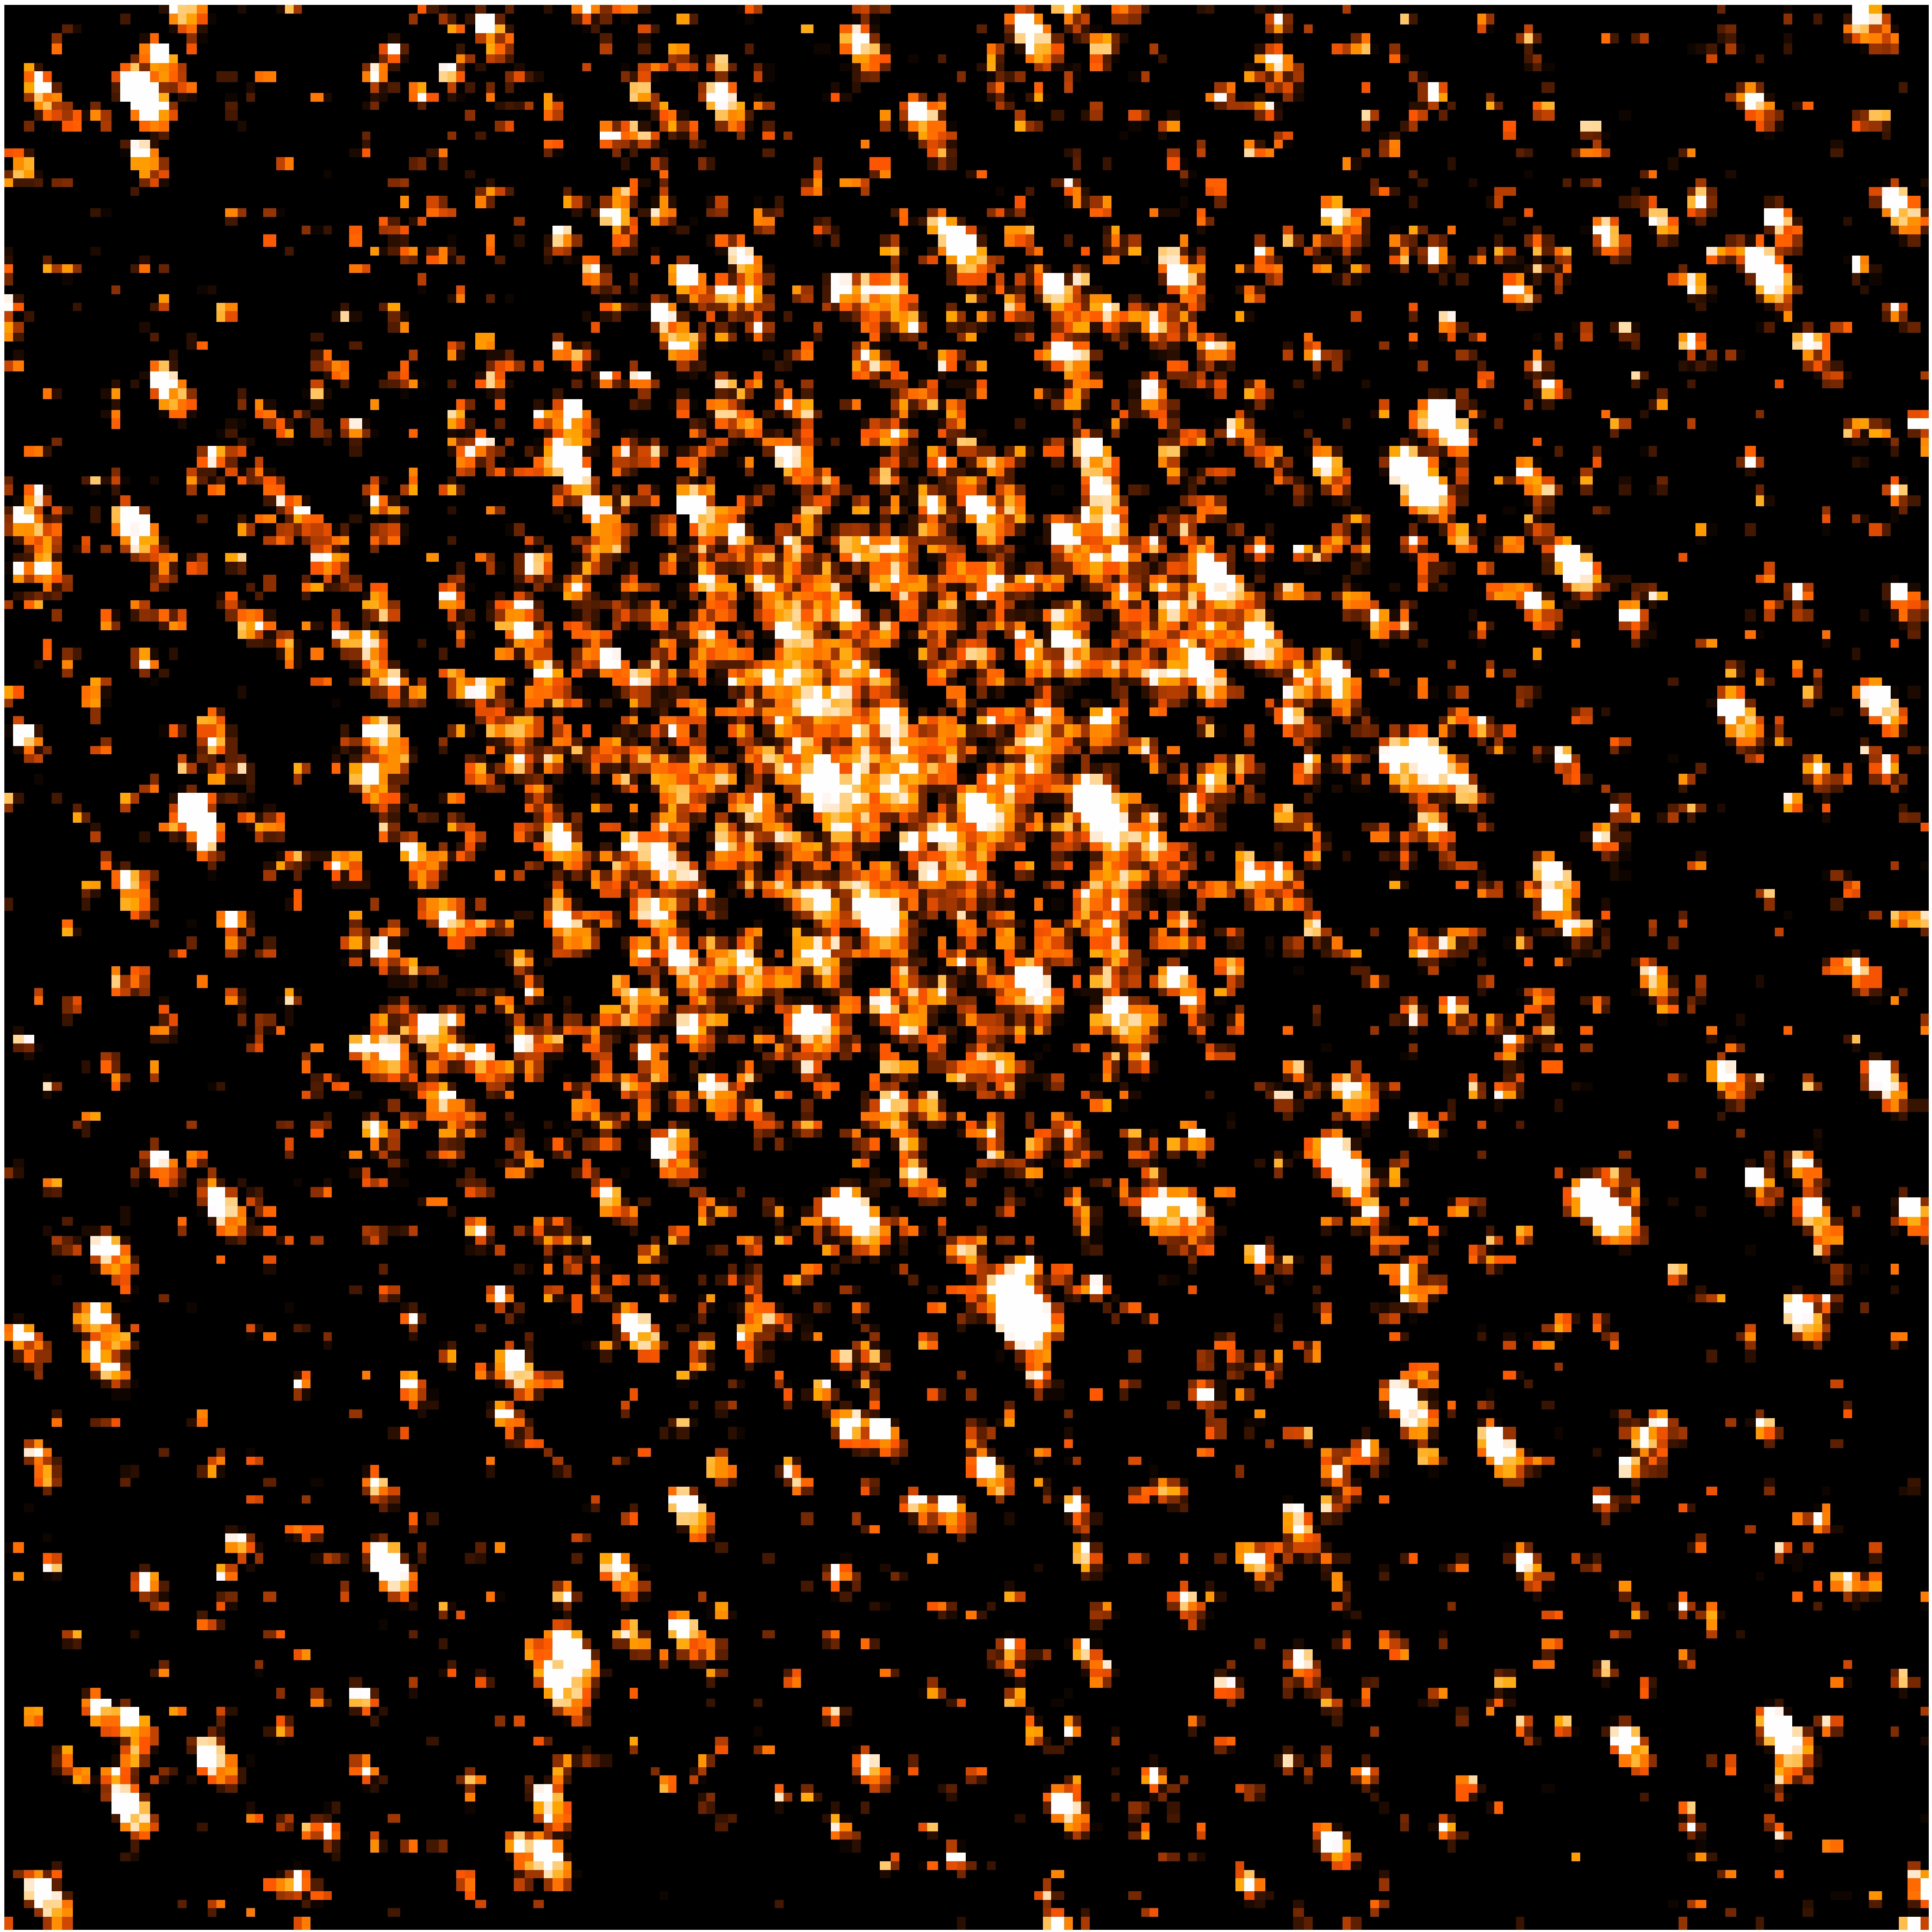
\includegraphics[width=0.45\linewidth]{Chapter1/ngc6791.jpg}
    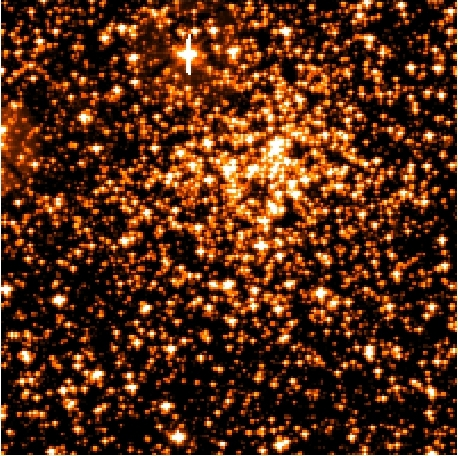
\includegraphics[width=0.45\linewidth]{Chapter1/ngc6819.jpeg}
    \caption[Superstamps of NGC\,6791 and NGC\,6819]{Typical exposures for superstamp images of the cores of the open clusters NGC\,6791 (left) and NGC\,6819 (right).}
    \label{fig:SS}
\end{figure}



%From honours thesis:
%"long, well-sampled time series with high accuracy in the measurements, are also critical for asteroseismic studies."
 




% Murphy Thesis
% Asteroseismology is the most informative method with which we can observe the
% stellar interior. Other than solar neutrinos, it is the only method. Oscillation fre-
% quencies present in stars’ light curves are the fundamental data of asteroseismology,
% and permit us to fine-tune stellar models. Although ground-based support is still
% required, particularly in constraining stellar atmospheric parameters and for direct
% mode identification, the existence of nearly continuous, micromagnitude-precision,
% space-based photometry is revolutionising our capacity to study stars.


%----------------------------------------------------------------------------------------------------------------------------------------------------------------
%----------------------------------------------------------------------------------------------------------------------------------------------------------------


\section{Photometric methods}



% Techniques for studying
% > CCDs - Simple ap phot
%       - PS phot
%       - Image sub

\subsection{Simple aperture photometry (SAP)}

\subsection{Point spread function (PSF) photometry}
Also known sometimes as pixel response function (PRF) photometry.

\subsection{Image Subtraction}